\chapter{Análises estatísticas}

% \textcolor{red}{Profs, eu ainda não consegui escrever sobre isso, mas a minha intenção nesse capítulo é correlacionar quais variáveis tem mais impacto em cada uma das visualizações, focando em quais delas seriam mais preditíveis segundo a análise dos algoritmos do capitulo anterior, conseguindo fechar na conclusão qual seria a melhor métrica possível pro SAP}

Para se compreender a relevância estatística significativa tanto das dimensões quanto dos fatores nas possíveis influências das variáveis socioeconômicas observadas no Capítulo \ref{cap:analises-sap}, foi decidido traçar o valor p (ou p-valor) para cada uma delas. Essa é uma medida estatística que ajuda a avaliar a significância estatística de um resultado em um teste de hipótese, então o valor p é a probabilidade de observar um resultado igual ou mais extremo do que o observado, sob a suposição de que a hipótese nula é verdadeira.

Para se calcular o valor p, é necessário primeiro traçar qual é a Hipótese Nula (H0), que é uma afirmação que assume que não há efeito ou diferença significativa; o valor p é usado para testar a validade da hipótese nula. Depois, traça-se a Hipótese Alternativa (H1), que é a afirmação que se deseja testar, sugerindo que existe uma diferença ou efeito significativo. Um valor p baixo (geralmente < 0,05) sugere que os resultados observados são improváveis de ocorrer sob a hipótese nula, levando à rejeição da hipótese nula. Um valor p alto indica que os resultados observados são plausíveis sob a hipótese nula, e não há evidências suficientes para rejeitá-la. Caso o valor p for menor que o nível de significância, rejeitamos a hipótese nula. Se o valor p for maior, não temos evidências suficientes para rejeitar a hipótese nula.

Para analisar essas relações das variáveis socioeconômicas com as dimensões e fatores, as Tabelas \ref{tab:pvalor_dimensao} e \ref{tab:pvalor_fatores} foram construídas. Elas apresentam os p-valores em destaque para todos os resultados menores que $0.05$, ou seja, os resultados com significância estatística. Então, analisando a Tabela \ref{tab:pvalor_dimensao}, é notável que os valores de p variam significativamente entre as diferentes variáveis, indicando que a associação entre essas variáveis e as dimensões ou fatores não é uniforme. Observa-se que, para a dimensão E\_ESCV (Estudante-Escola), o sexo não apresenta uma associação significativa, enquanto o ``porte\_da\_escola'' e ``id\_renda\_familiar'' mostram uma associação forte com p-valores muito baixos. Isso sugere que características como o tamanho da escola e a renda familiar têm um impacto mais significativo na dimensão relacionada à escola. No contexto da dimensão E\_PROFV (Profissionais da Escola), o sexo tem um p-valor muito baixo, indicando uma associação significativa. Além disso, ``ano\_turma'' e ``outras\_ofertas\_educacionais'' também apresentam p-valores baixos, sugerindo uma associação considerável com essa dimensão.

Para a dimensão E\_FAMV (Estudante-Família), vários fatores, como ``sexo'', ``uf'', ``localizacao'', ``ano\_turma'', ``localidade\_diferenciada'', ``dependencia\_administrativa'', ``id\_raca\_etnia'', ``porte\_da\_escola'', ``outras\_ofertas\_educacionais'' e ``id\_renda\_familiar'', mostram p-valores muito baixos. Isso sugere que esses fatores estão fortemente associados à dimensão relacionada à família. Ao examinar a dimensão E\_COMV (Estudante-Comunidade), quase todas as variáveis têm p-valores muito baixos, indicando associações significativas. Notavelmente, ``sexo'' e ``ano\_turma'' têm p-valores mais elevados, sugerindo uma menor associação com essa dimensão. Por fim, para a dimensão E\_ESTV (Estudante-Estudante), vários fatores apresentam p-valores altos, indicando uma associação menos significativa. ``sexo'', ``localizacao'', ``ano\_turma'', ``localidade\_diferenciada'', ``dependencia\_administrativa'', ``id\_raca\_etnia'', ``porte\_da\_escola'', ``outras\_ofertas\_educacionais'' e ``id\_renda\_familiar'' têm p-valores relativamente altos, sugerindo que esses fatores podem ter uma influência menos acentuada na dimensão do estudante. 

\begin{table}[ht!]
    \centering
    \caption{P Valor relacionado às Dimensões}
    \resizebox{\textwidth}{!}{%
    \begin{tabular}{|c|c|c|c|c|c|c|c|c|c|c|}
        \hline
        \textbf{} &
          \textbf{sexo} &
          \textbf{uf} &
          \textbf{localizacao} &
          \textbf{ano\_turma} &
          \textbf{\begin{tabular}[c]{@{}c@{}}localidade\_\\ diferenciada\end{tabular}} &
          \textbf{\begin{tabular}[c]{@{}c@{}}dependencia\_\\ administrativa\end{tabular}} &
          \textbf{\begin{tabular}[c]{@{}c@{}}id\_raca\_\\ etnia\end{tabular}} &
          \textbf{\begin{tabular}[c]{@{}c@{}}porte\_da\\ \_escola\end{tabular}} &
          \textbf{\begin{tabular}[c]{@{}c@{}}outras\_ofertas\\ \_educacionais\end{tabular}} &
          \textbf{\begin{tabular}[c]{@{}c@{}}id\_renda\_\\ familiar\end{tabular}} \\ \hline
        \textbf{E\_ESCV}  & 0.039 & 0.938 & 0.486 & 0.372 & 0.066 & 0.568 & 0.141 & \textbf{0.000} & 0.201 & \textbf{0.000} \\ \hline
        \textbf{E\_PROFV} & \textbf{0.000 }& 0.141 & \textbf{0.010} & \textbf{0.025} & 0.579 & \textbf{0.000} & 0.951 & \textbf{0.041} & \textbf{0.000} & 0.150 \\ \hline
        \textbf{E\_FAMV}  & \textbf{0.000} & \textbf{0.075} & \textbf{0.000} & \textbf{0.000} & \textbf{0.000} & 0.050 & \textbf{0.028} & \textbf{0.000} & \textbf{0.000} & \textbf{0.000} \\ \hline
        \textbf{E\_COMV}  & \textbf{0.000} & \textbf{0.000} & \textbf{0.000} & \textbf{0.000} & \textbf{0.002} & \textbf{0.000} & \textbf{0.002} & \textbf{0.000} & 0.239 & \textbf{0.000} \\ \hline
        \textbf{E\_ESTV}  & 0.213 & \textbf{0.030} & 0.538 & 0.668 & 0.850 & 0.514 & 0.844 & 0.249 & 0.411 & 0.594 \\ \hline
    \end{tabular}%
    }
    \label{tab:pvalor_dimensao}
    \fonte{\me{2023}}
\end{table}

\begin{table}[ht!]
    \centering
    \caption{P Valor relacionado aos Fatores}
    \resizebox{\textwidth}{!}{%
    \begin{tabular}{|c|c|c|c|c|c|c|c|c|c|c|}
        \hline
        \textbf{} &
          \textbf{sexo} &
          \textbf{uf} &
          \textbf{localizacao} &
          \textbf{ano\_turma} &
          \textbf{\begin{tabular}[c]{@{}c@{}}localidade\_\\ diferenciada\end{tabular}} &
          \textbf{\begin{tabular}[c]{@{}c@{}}dependencia\_\\ administrativa\end{tabular}} &
          \textbf{\begin{tabular}[c]{@{}c@{}}id\_raca\_\\ etnia\end{tabular}} &
          \textbf{\begin{tabular}[c]{@{}c@{}}porte\_da\\ \_escola\end{tabular}} &
          \textbf{\begin{tabular}[c]{@{}c@{}}outras\_ofertas\\ \_educacionais\end{tabular}} &
          \textbf{\begin{tabular}[c]{@{}c@{}}id\_renda\_\\ familiar\end{tabular}} \\ \hline
        \textbf{E\_ESC1V}  & \textbf{0.011} & 0.079 & 0.465 & 0.305 & 0.416 & \textbf{0.000} & \textbf{0.020} & 0.748 & 0.083 & \textbf{0.032} \\ \hline
        \textbf{E\_ESC2V}  & \textbf{0.001} & 0.064 & 0.109 & 0.199 & 0.138 & \textbf{0.009} & 0.935 & \textbf{0.000} & \textbf{0.002} & \textbf{0.000} \\ \hline
        \textbf{E\_PROF1V} & 0.533 & 0.177 & \textbf{0.015} & 0.061 & 0.116 & \textbf{0.000} & 0.385 & 0.713 & 0.443 & \textbf{0.000} \\ \hline
        \textbf{E\_PROF2V} & \textbf{0.000} & 0.116 & 0.383 & 0.236 & 0.717 & \textbf{0.000} & 0.369 & 0.706 & \textbf{0.000} & 0.079 \\ \hline
        \textbf{E\_FAM1V}  & \textbf{0.000} & 0.159 & 0.093 & \textbf{0.000} & \textbf{0.000} & \textbf{0.000} & \textbf{0.004} & \textbf{0.000} & \textbf{0.000} & 0.065 \\ \hline
        \textbf{E\_FAM2V}  & \textbf{0.001} & 0.612 & \textbf{0.000} & 0.803 & \textbf{0.024} & \textbf{0.000} & 0.627 & 0.865 & 0.245 & \textbf{0.000} \\ \hline
        \textbf{E\_COM1V}  & \textbf{0.000} & \textbf{0.000} & \textbf{0.000} & 0.330 & \textbf{0.000} & \textbf{0.000} & 0.641 & 0.415 & \textbf{0.000} & \textbf{0.000} \\ \hline
        \textbf{E\_COM2V}  & \textbf{0.000} & 0.074 & 0.701 & \textbf{0.000} & 0.500 & 0.182 & 0.285 & 0.276 & 0.820 & 0.835 \\ \hline
        \textbf{E\_COM3V}  & 0.095 & 0.781 & \textbf{0.000} & 0.240 & 0.938 & \textbf{0.000} & 0.339 & 0.527 & \textbf{0.025} & 0.648 \\ \hline
        \textbf{E\_EST1V}  & \textbf{0.000} & 0.988 & \textbf{0.000} & 0.215 & 0.307 & \textbf{0.000} & 0.804 & \textbf{0.028} & 0.632 & \textbf{0.002} \\ \hline
        \textbf{E\_EST2V}  &\textbf{ 0.000} &\textbf{ 0.000} & 0.060 & \textbf{0.000} & 0.332 & \textbf{0.001} & 0.127 & 0.409 & \textbf{0.003} & 0.000 \\ \hline
        \textbf{E\_EST3V}  & 0.069 & \textbf{0.000} & \textbf{0.001} & \textbf{0.000} & 0.009 & \textbf{0.001} & \textbf{0.033} & \textbf{0.015} &\textbf{ 0.006} & 0.057 \\ \hline
    \end{tabular}%
    }
    \label{tab:pvalor_fatores}
    \fonte{\me{2023}}
\end{table}

Então, observa-se que as variáveis socioeconômicas possuem um impacto distinto nos fatores e dimensões, com algumas se relacionando com mais áreas que outras. Portanto, para melhor observar essa relação, foram selecionadas as variáveis socieconômicas que se relacionaram com o maior número de dimensões e fatores, as quais são elas:

\begin{itemize}
    \item Dimensões: porte\_da\_escola, com 4 relações; e sexo, uf, localizacao, ano\_turma e id\_renda\_familiar com 3 relações cada;
    \item Fatores: dependencia\_administrativa com 11 relações; e sexo, com 9 relações.
\end{itemize}

Visando observar alguns dos comportamentos de relação entre as variáveis listadas que possuem o maior número de relações com os Fatores e Dimensões, os gráficos das Figuras \ref{fig:porte_escola}, \ref{fig:sexo}, \ref{fig:localizacao_dimensao}, \ref{fig:renda-dimensoes}, \ref{fig:fat-dependencia} e \ref{fig:sexo_fatores}, apresentam a relação entre as dimensões e o porte da escola, sexo, localizacao, ano da turma e renda familiar, respectivamente. Já as Figuras \ref{fig:fat-dependencia} e \ref{fig:sexo_fatores} relacionam os fatores com a dependência administrativa e o sexo dos estudantes, respectivamente. É importante salientar que, embora a UF seja uma variável com três relações com as dimensões, ela não será analisada em gráfico, visto que uma análise mais aprofundada da relação do estado do estudante com as dimensões necessitaria de dados mais balanceados, já que, como apresentado na Figura \ref{fig:uf}, a diferença da quantidade de estudantes que responderam à pesquisa entre um estado e outro pode ser de até 5101. Há ainda estados que não foram representados, como é o caso, por exemplo, do Paraná e Acre.

A Figura \ref{fig:porte_escola} apresenta a relação que cada um dos valores das dimensões E\_ESCV, E\_PROFV, E\_FAMV e E\_COMV tem com os estudantes de portes de escola diferentes. Nesta imagem, é possível observar que há uma disparidade na quantidade de estudantes de cada tipo de escola, com as escolas entre 201 e 500 matrículas possuindo a maioria dos estudantes para todos os valores das dimensões. Para a dimensão E\_ESCV observa-se que as notas mais altas, como 6 e 7 possuem uma porcentagem maior de estudantes de escolas entre 501 e 1000 matrículas do que se comparado com os valores mais baixos. Já para E\_PROFV acontece o fenômeno inverso, e esse porte de escola possui uma menor porcentagem de estudantes nas notas 6 e 7 do que nas demais notas. Além disso, a porcentagem de estudantes das escolas de porte de até 50 matrículas e de 201 a 500 matrículas atingem seus máximos na nota 7 de E\_PROFV. Outro ponto de destaque é o gráfico para E\_FAMV, que 100\% dos alunos que responderam a maior nota para essa dimensão eram de escolas de porte de 51 a 200 matrículas.

\begin{figure}[ht!]
    \centering
    \caption{Correlação entre dimensões e porte da escola}
    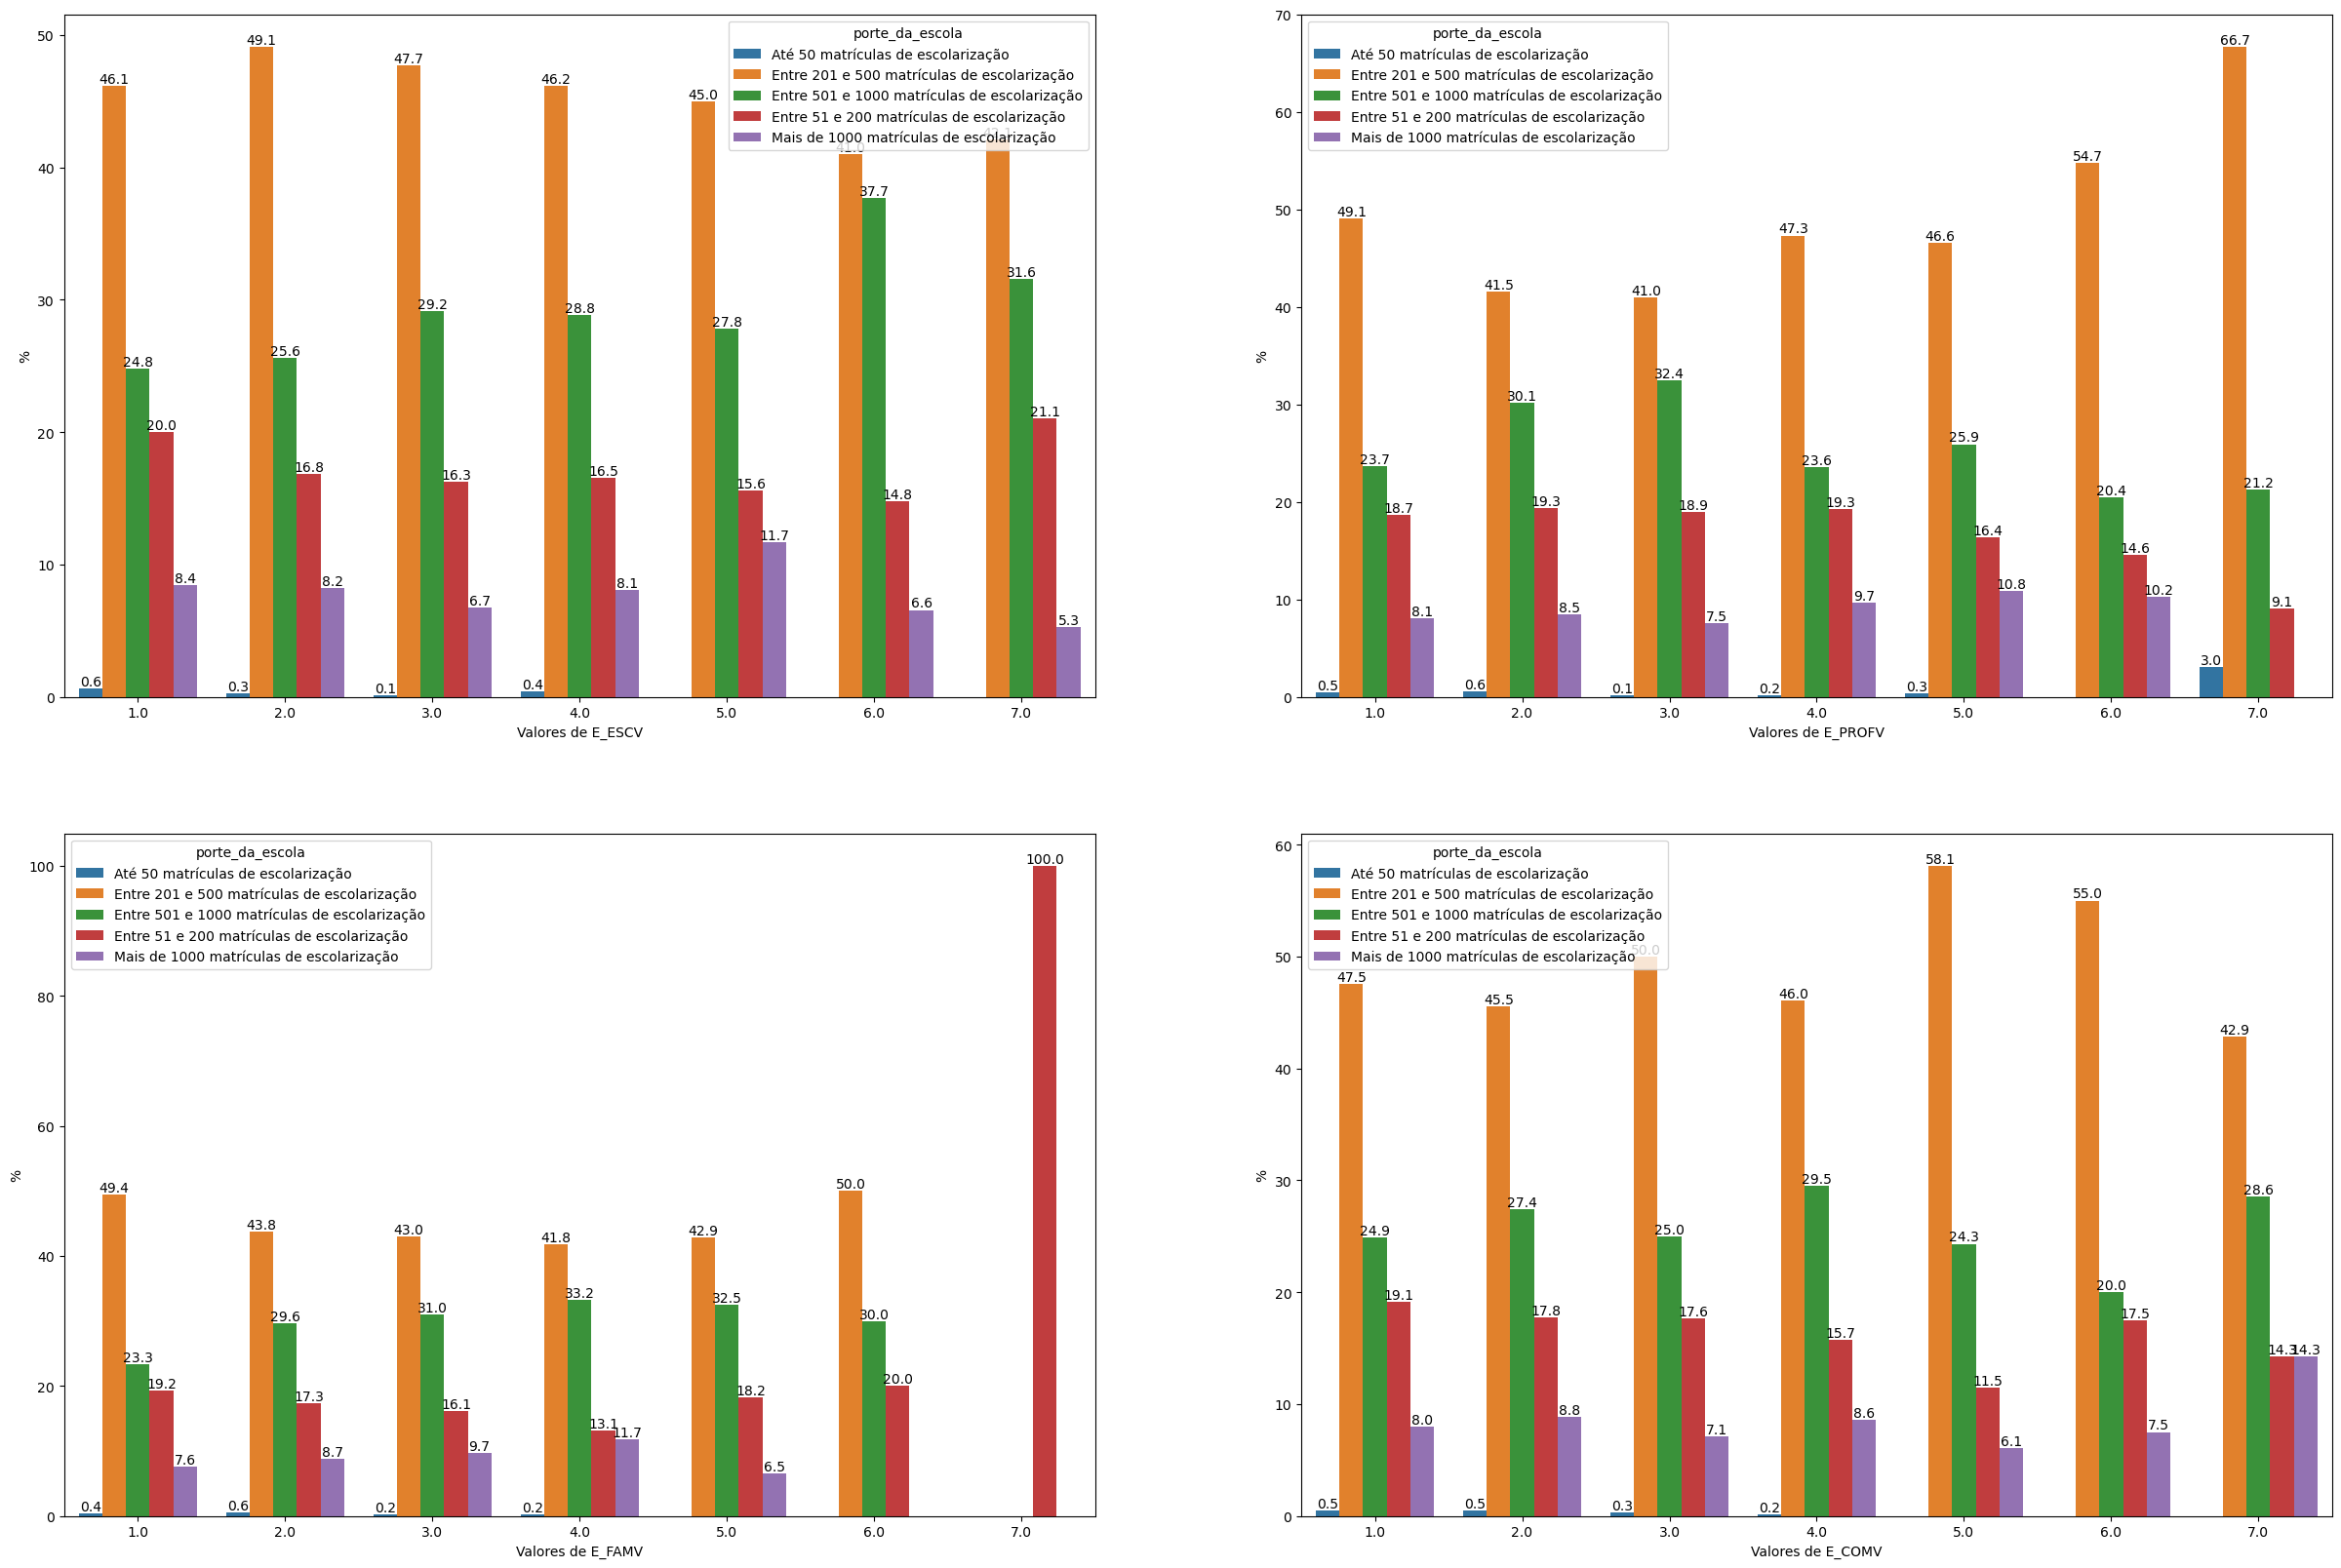
\includegraphics[width=1\textwidth]{Textuais/Imagens/Filé/porte_escola.png}
    \label{fig:porte_escola}
    \fonte{\me{2023}}
\end{figure}

 Na Figura \ref{fig:sexo} é possível notar que valores mais altos das dimensões E\_PROFV, E\_FAMV e E\_COMV apresentam uma porcentagem maior de estudantes homens do que mulheres, o que foi observado como sendo uma diferença significativa pelo p-valor. Essa diferença é especialmente grande para a dimensão E\_FAMV, onde 100\% dos alunos que obtiveram o valor 7.0 eram do sexo masculino.


\begin{figure}[ht!]
    \centering
    \caption{Correlação entre dimensões e sexo}
    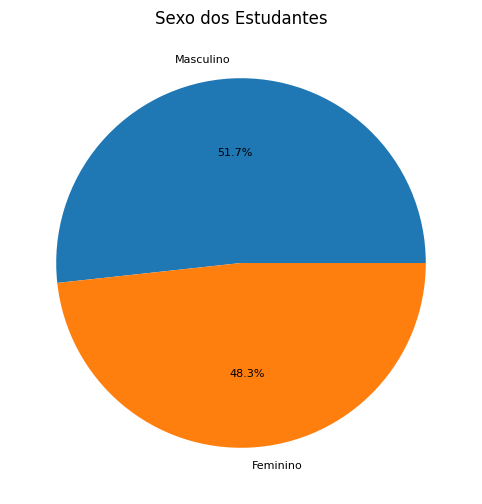
\includegraphics[width=1\textwidth]{Textuais/Imagens/Filé/sexo.png}
    \label{fig:sexo}
    \fonte{\me{2023}}
\end{figure}

% \begin{figure}[ht!]
%     \centering
%     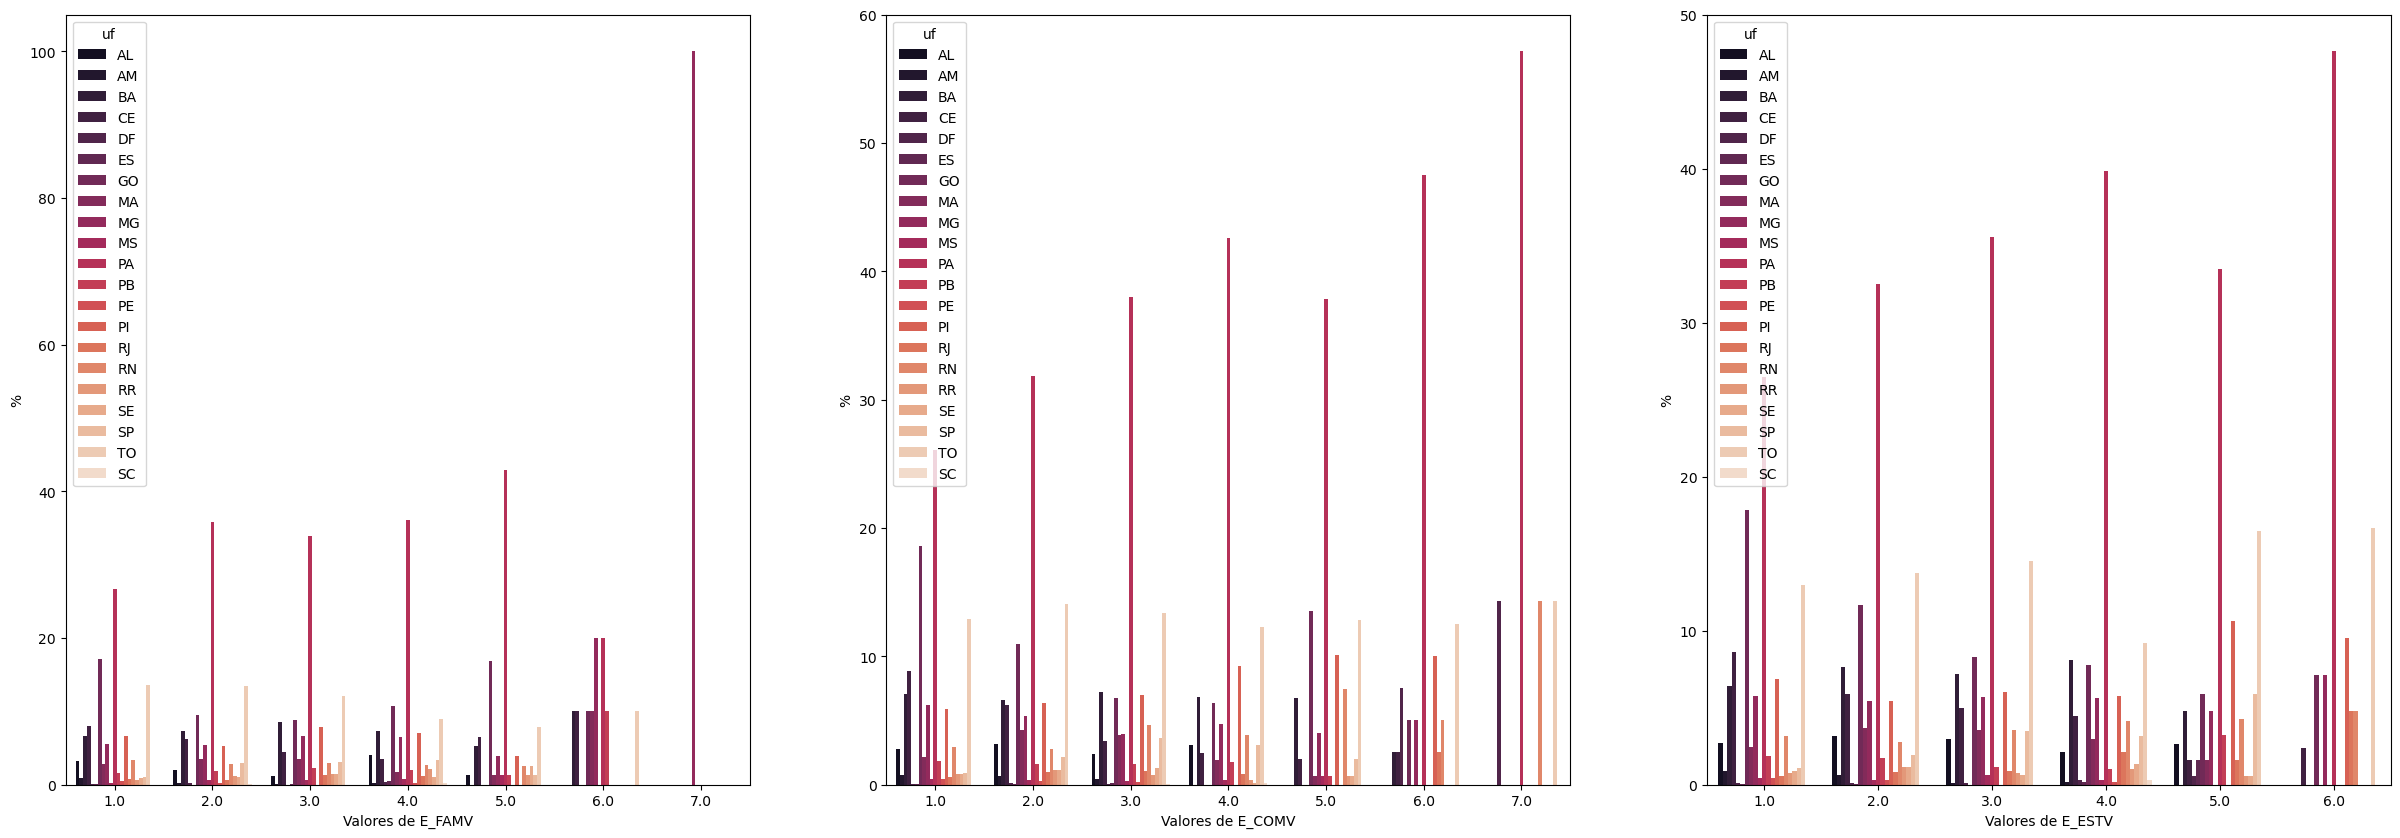
\includegraphics[width=1\textwidth]{Textuais/Imagens/Filé/uf.png}
%     \caption{Correlação entre dimensões e Unidade Federativa}
%     \label{fig:uf-dim}
% \end{figure}

A relação entre as dimensões E\_PROFV, E\_FAMV e E\_COMV e a localização dos estudantes pode ser vista na Figura \ref{fig:localizacao_dimensao}. Nela, é notável a porcentagem maior de estudantes na região urbana que possuem a nota mais alta para as dimensões analisadas, se comparado com estudantes da região rural.

\begin{figure}[ht!]
    \centering
    \caption{Correlação entre dimensões e localização}
    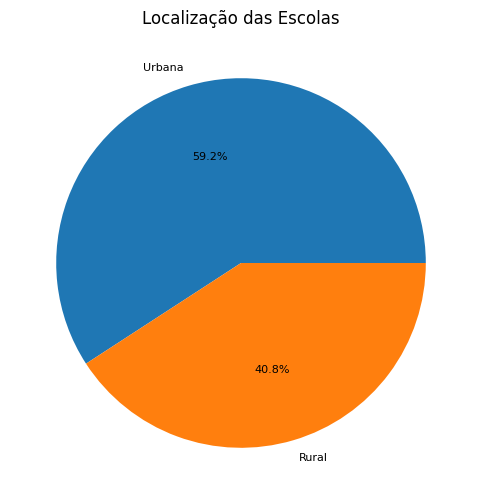
\includegraphics[width=1\textwidth]{Textuais/Imagens/Filé/localizacao.png}
    \label{fig:localizacao_dimensao}
    \fonte{\me{2023}}
\end{figure}

A Figura \ref{fig:renda-dimensoes} apresenta a relação entre a renda familiar do estudante e os fatores E\_ESCV, E\_FAMV e E\_COMV. Nela, é possível perceber que para os fatores E\_ESCV e E\_COMV, não há nenhum estudante que obteve as notas 6 e 7 cuja renda familiar é superior a 7 salários mínimos. Para a dimensão E\_FAMV, o valor 7 foi respondido 100\% por estudantes cuja renda familiar é de até um salário mínimo. Ainda, um ponto de destaque é que a nota 6 teve um pico de estudantes cuja renda familiar é superior a 9 salários mínimos.


\begin{figure}[ht!]
    \centering
    \caption{Correlação entre dimensões e renda familiar}
    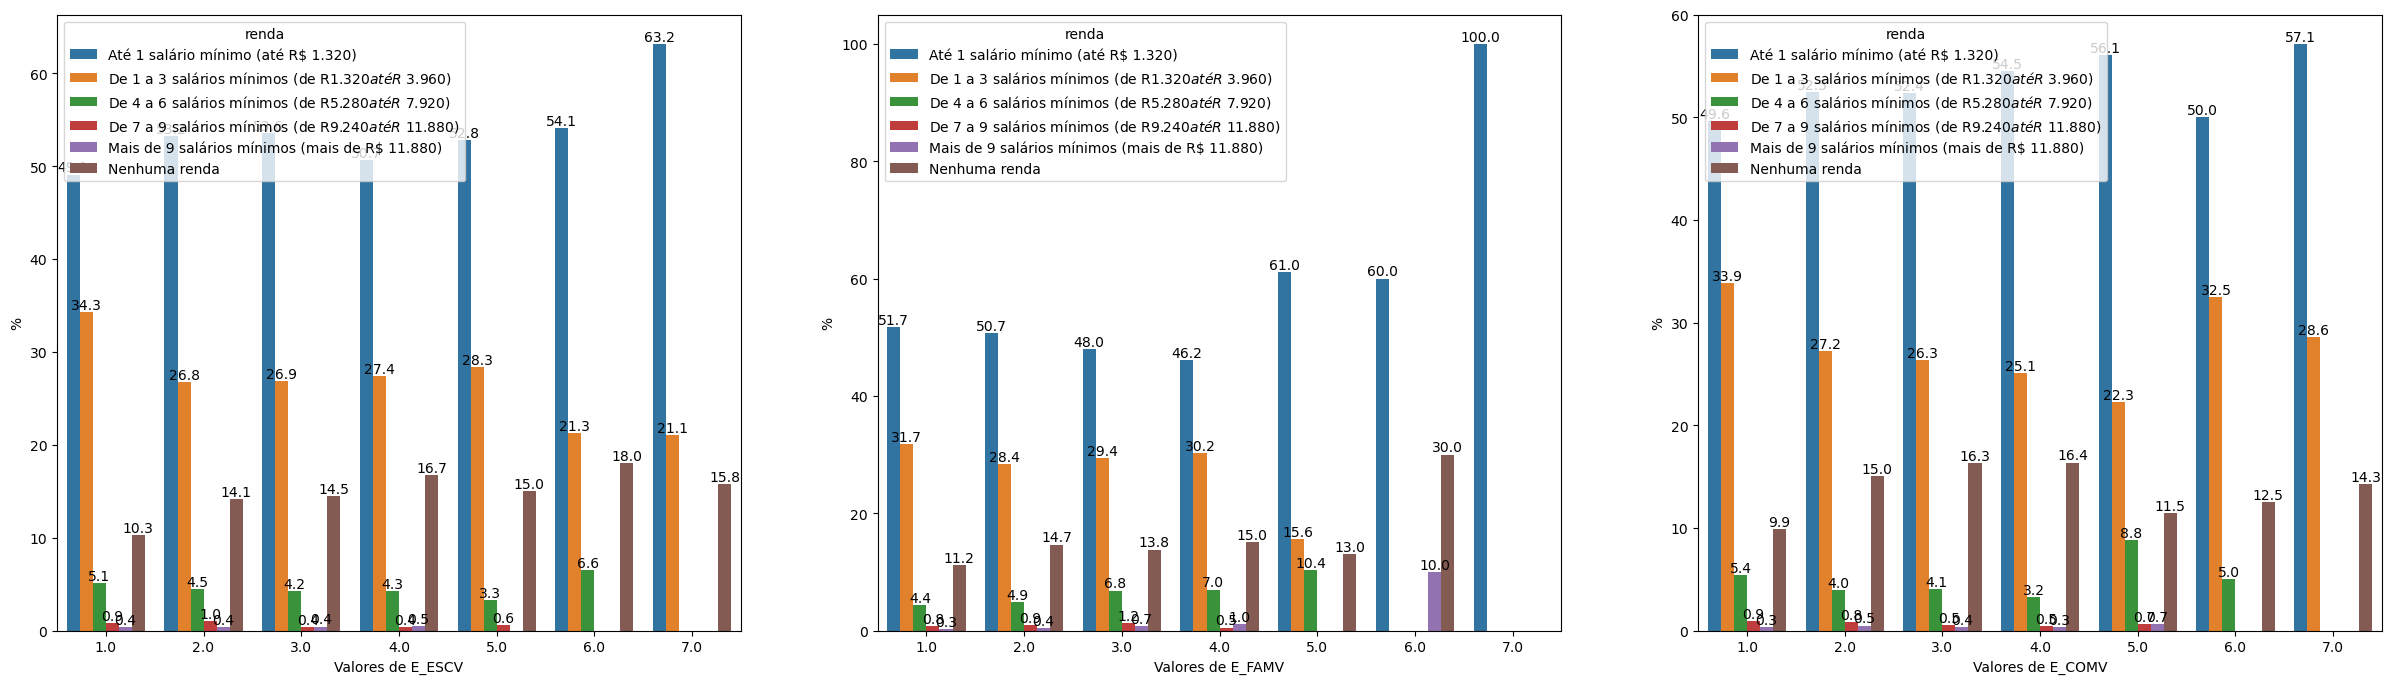
\includegraphics[width=1\textwidth]{Textuais/Imagens/Filé/renda.png}
    \label{fig:renda-dimensoes}
    \fonte{\me{2023}}
\end{figure}

Para a análise dos fatores, a Figura \ref{fig:fat-dependencia} apresenta a relação entre a dependência administrativa da escola do estudante com uma série de fatores distintos, cuja relação é significativa, conforme o p-valor observado. Com isso, alguns pontos de destaque desta relação são encontrados nos fatores E\_COM1V (Medidas Socioeducativas e Contextos de Violência), E\_EST3V (Reprovações e Distorção Idade – Série), onde a medida que a nota aumenta, a porcentagem de estudantes de escolas municipais aumenta e de escolas estaduais diminui. Outro ponto de destaque é o fator E\_FAM1V (Suporte Familiar), que para a nota 7, 100\% dos estudantes eram de escolas estaduais.


\begin{figure}[ht!]
    \centering
    \caption{Correlação entre fatores e dependência administrativa}
    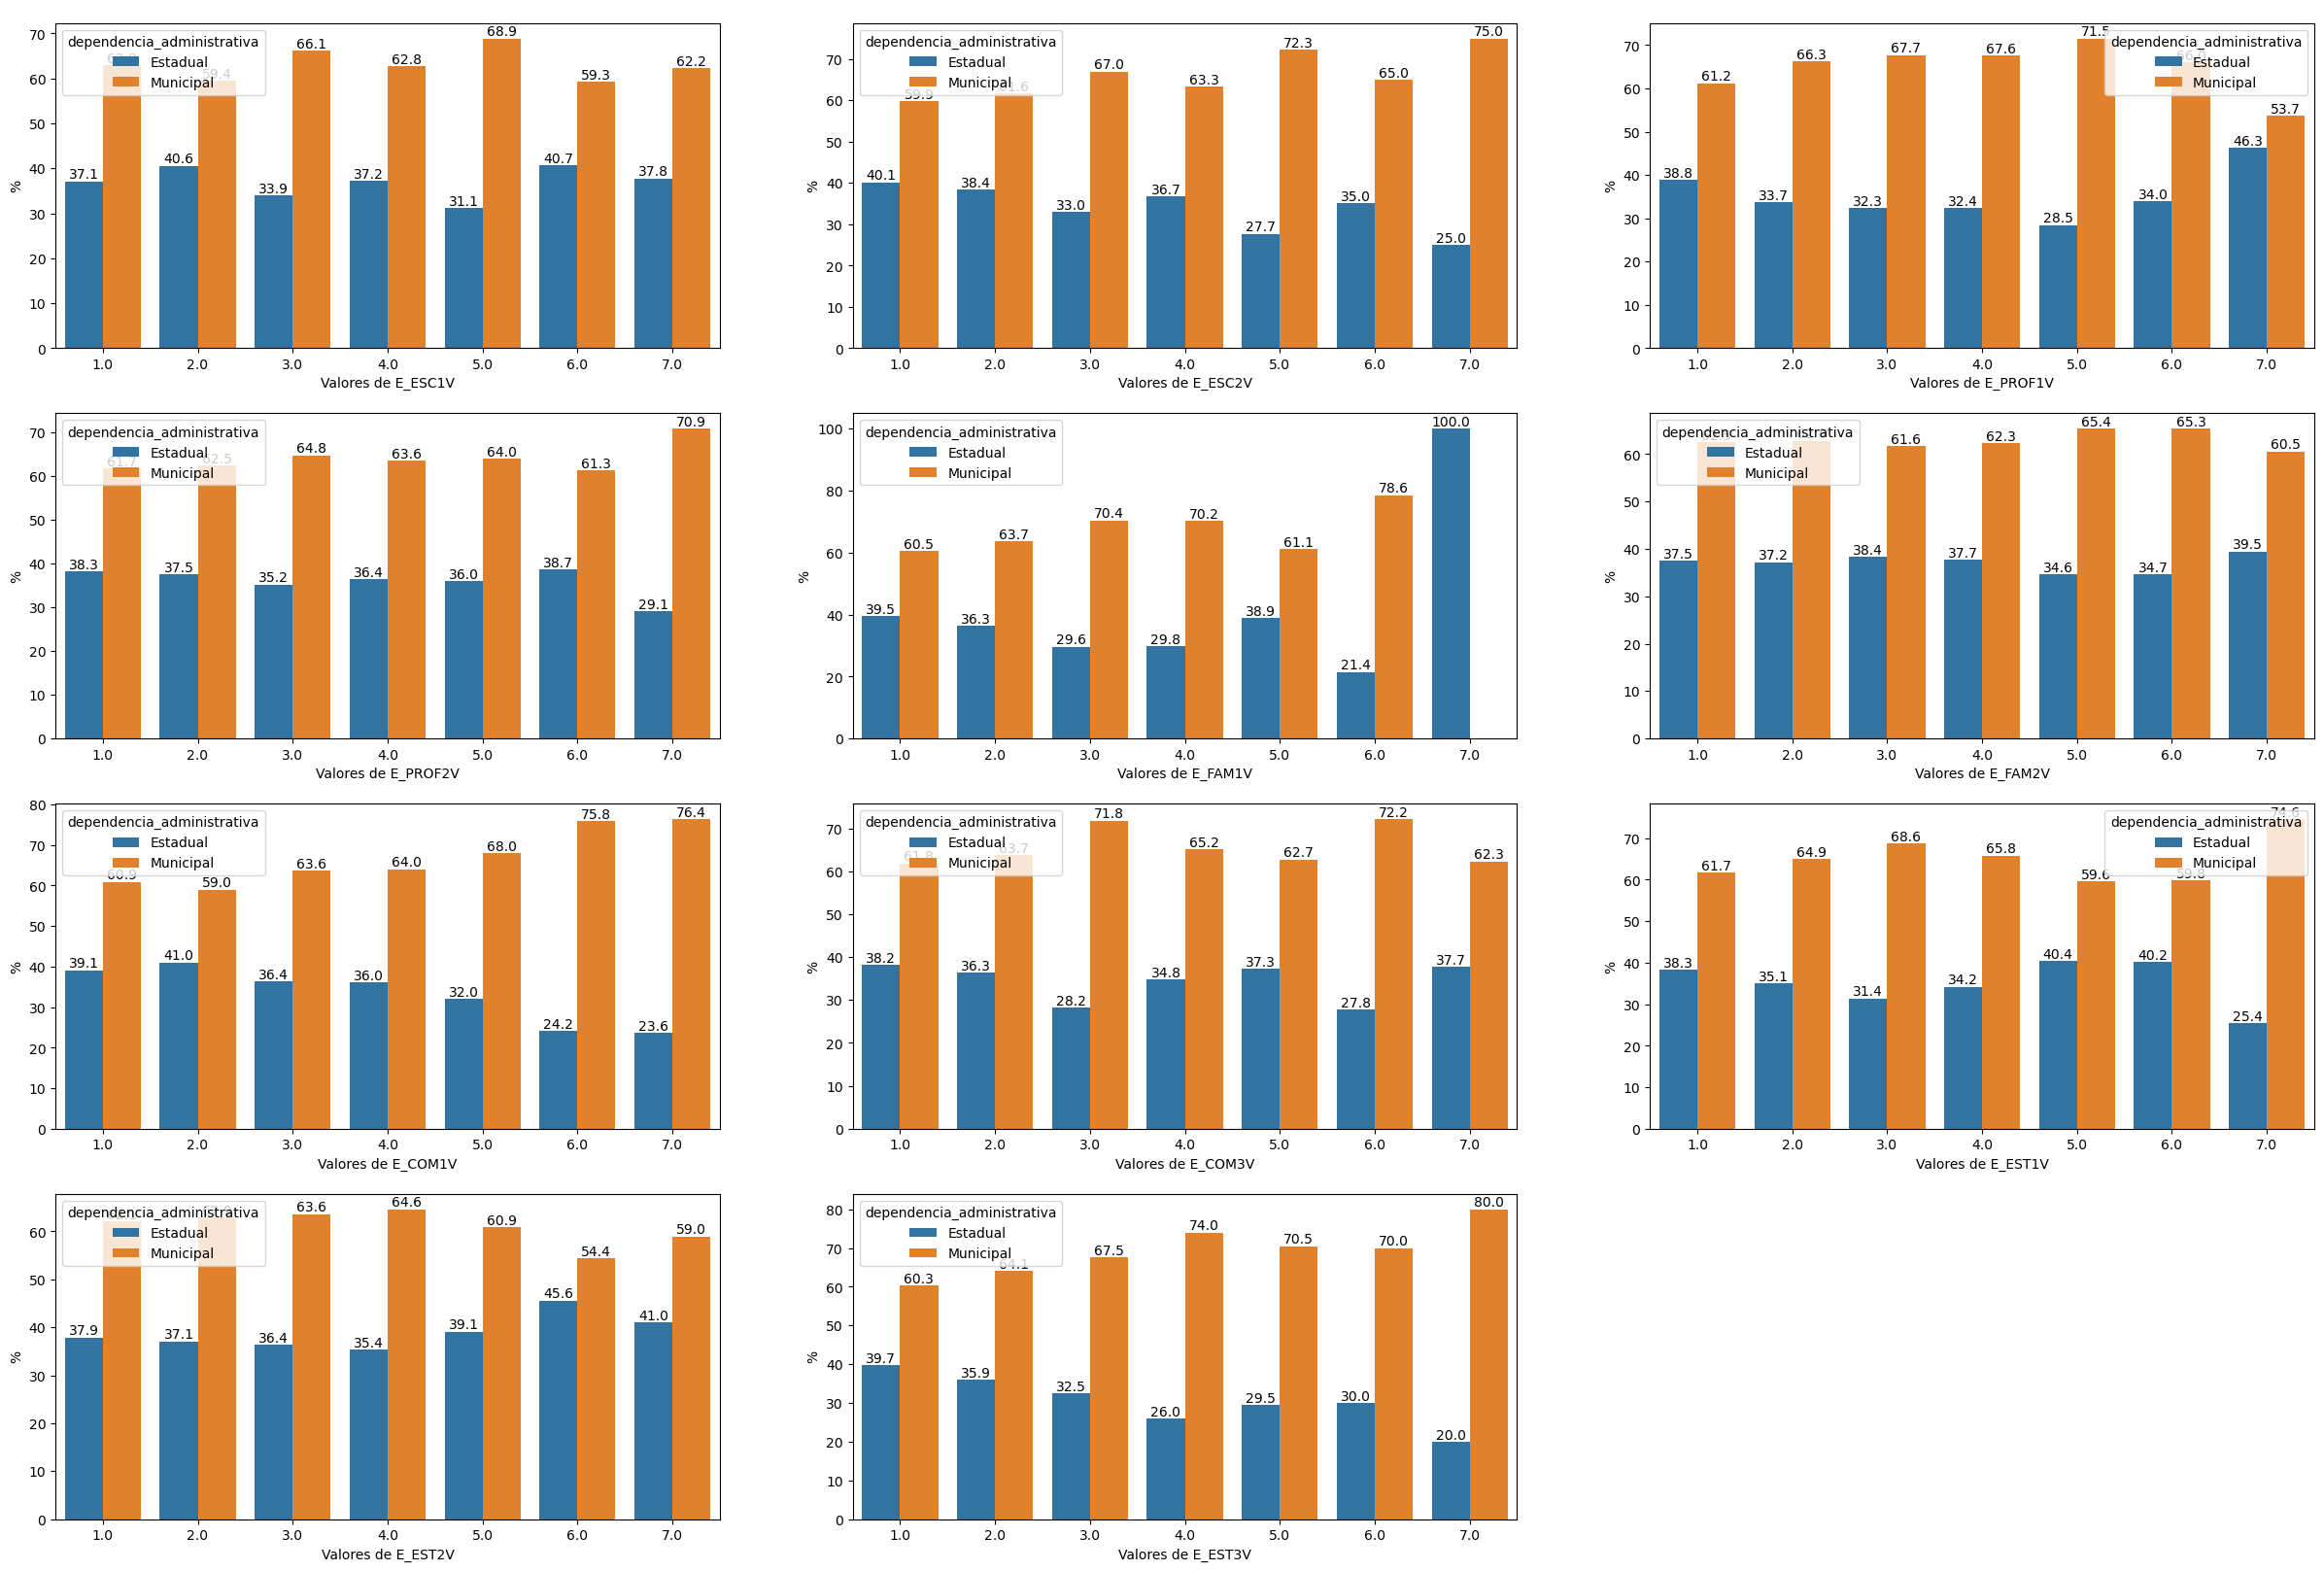
\includegraphics[width=1\textwidth]{Textuais/Imagens/Filé/dependencia_admin.png}
    \label{fig:fat-dependencia}
    \fonte{\me{2023}}
\end{figure}


Por fim, a Figura \ref{fig:sexo_fatores} apresenta a relação de fatores diversos com a variável sexo. Nela, os fatores E\_ESC2V (Condições Materiais do(a) Estudante) e E\_COM1V (Medidas Socioeducativas e Contextos de Violência) apresentam uma queda clara da porcentagem de estudantes do sexo feminino em detrimento do aumento dos estudantes do sexo masculino à medida que a nota para esses fatores aumenta. Outro ponto de interesse acontece no fator E\_FAM1V que para a nota 7, 100\% dos estudantes são do sexo masculino.


\begin{figure}[ht!]
    \centering
    \caption{Correlação entre fatores e sexo}
    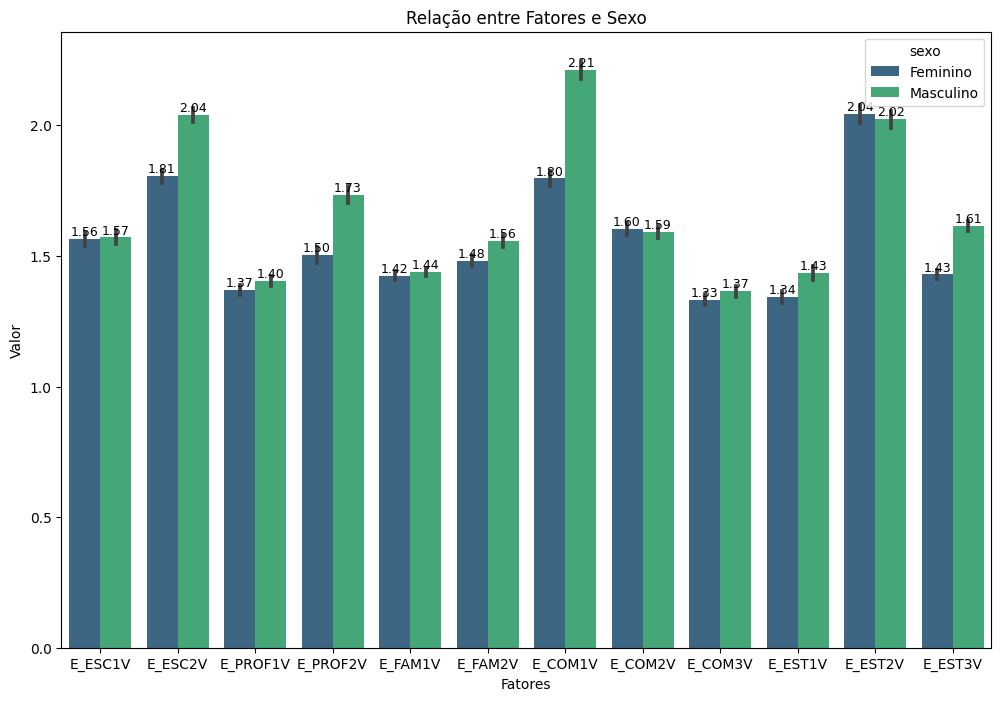
\includegraphics[width=1\textwidth]{Textuais/Imagens/Filé/sexo_fatores.png}
    \label{fig:sexo_fatores}
    \fonte{\me{2023}}
\end{figure}

No entanto, é possível notar que a distribuição de valores do número de estudantes de cada categoria é bastante desigual, com, por exemplo, uma porcentagem muito maior de estudantes do sexto, sétimo, oitavo e nono ano do que dos demais. Esse desbalanço, que ocorre em diversas variáveis sociodemográficas, pode ser um grande influenciador dos resultados obtidos para o p-valor.

Outra métrica analisada para identificar padrões de associação ou dependência entre as diferentes dimensões do conjunto de dados foi traçar uma análise de correlação entre as variáveis das dimensões e entre as variáveis dos fatores para analisar qual delas poderia ter mais influência uma sobre as outras. Essas matrizes de correlações são representadas pelas Figuras \ref{fig:matriz-correlacao-dimensoes} e \ref{fig:matriz-correlacao-fatores}. Nelas, é possível verificar que quando os números estão mais próximos de 1.0 significa que há uma maior correlação positiva entre as variáveis, e quando estão próximos de -1.0, há uma maior correlação negativa, com valores próximos a zero não possuindo muita significância. É importante lembrar que enquanto duas variáveis estão correlacionadas uma à outra, isso não significa que uma implica na causalidade da outra.

Tendo isso em mente, é notável na Figura \ref{fig:matriz-correlacao-dimensoes} a correlação positiva mediana que há entre as dimensões E\_PROFV e E\_COMV, com 0.41, atingindo o maior número dentre as dimensões. Ou seja, isso significa que há uma tendência de quando os valores de E\_COMV forem mais altos, há maior probabilidade de E\_PROFV também serem, indicando que há uma interligação entre esses dois fatores dentro do questionário. 

\begin{figure}[ht!]
    \centering
    \caption{Correlação entre dimensões}
    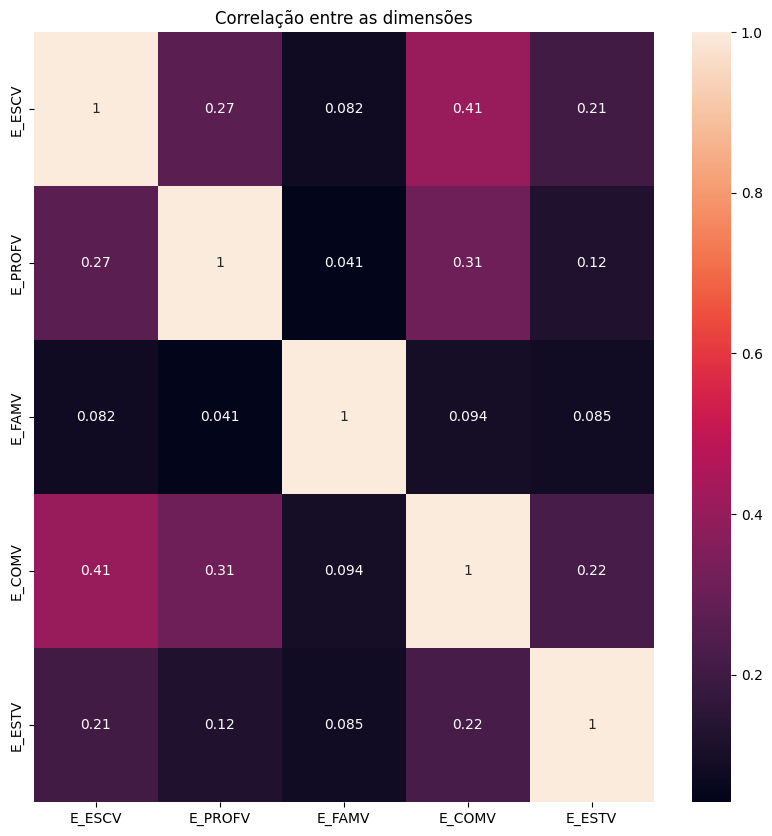
\includegraphics[width=0.7\textwidth]{Textuais/Imagens/Filé/correlacao_dimensoes.png}
    \label{fig:matriz-correlacao-dimensoes}
    \fonte{\me{2023}}
\end{figure}

Já na Figura \ref{fig:matriz-correlacao-fatores}, percebe-se que o fator E\_FAM1V (Suporte Familiar) é o que possui correlação negativa com a maioria todos os outros fatores, exceto com E\_EST3V (Reprovações e Distorção idade-série), o que indica que é uma variável significativa mesmo que inversamente proporcional às outras. É importante ressaltar que o fator E\_EST3V também possui em sua maioria correlação negativa com os outros fatores, mas são valores mais próximos de zero que a variável anterior, indicando que possui menos significância estatística correlacional. Nota-se também que os fatores E\_FAM2V (Gravidez/parentalidade/atividades de cuidado) e E\_COM2V (Acessibilidade e frequência escolar) são os que possuem maior correlação positiva com a maioria dos outros fatores, com seus valores positivos ficando entre 0.13 a 0.38 e 0.11 a 0.33, respectivamente.

\begin{figure}[ht!]
    \centering
    \caption{Correlação entre fatores}
    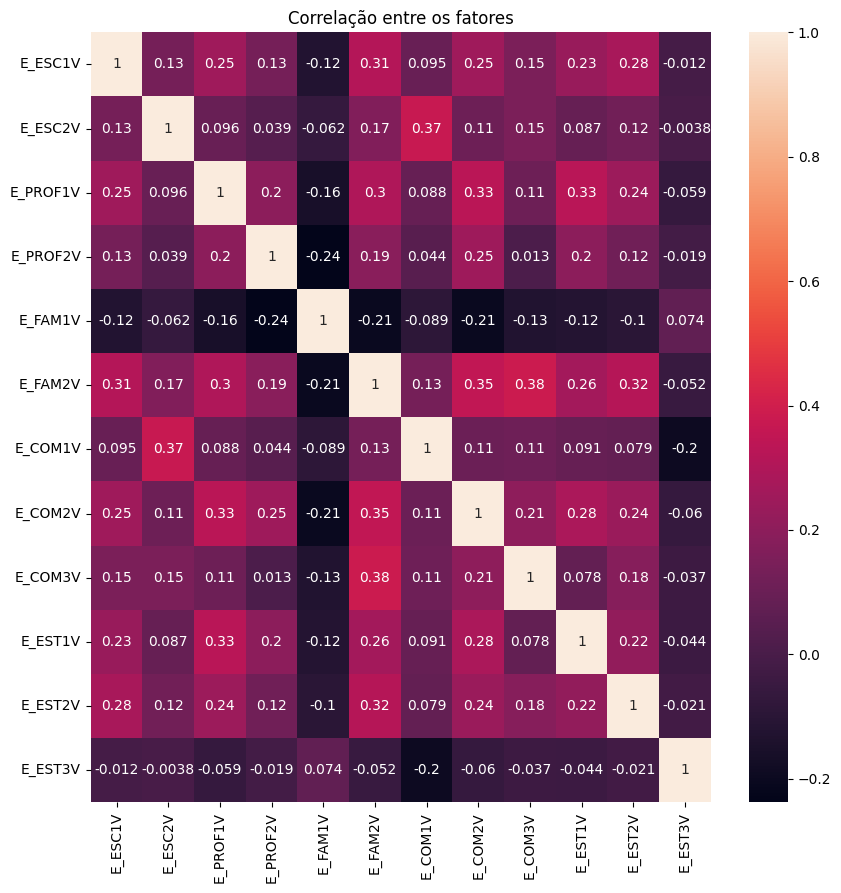
\includegraphics[width=0.8\textwidth]{Textuais/Imagens/Filé/correlacao_fatores.png}
    \label{fig:matriz-correlacao-fatores}
    \fonte{\me{2023}}
\end{figure}

Após as análises estatísticas feitas, o próximo passo da pesquisa são as análises classificatórias com o auxílio de \textit{machine learning}, a ser realizado no próximo capítulo.

%%%%%%%%%%%%%%%%%%%%%%%%%%%%%%%%%%%

% Por fim, foi decidido estudar o relacionamento das médias das dimensões e fatores em comparação com variáveis estatísticas exclusivas dos estudantes, resultando nos gráficos das Figuras \ref{fig:dimensoes-etnia}, \ref{fig:fatores-etnia}, \ref{fig:dimensoes-sexo}, \ref{fig:fatores-sexo}, \ref{fig:dimensoes-anoensino}, \ref{fig:fatores-anoensino}, \ref{fig:dimensoes-anoensino-radar} e \ref{fig:fatores-anoensino-radar}.

% \begin{figure}[ht!]
%     \centering
%     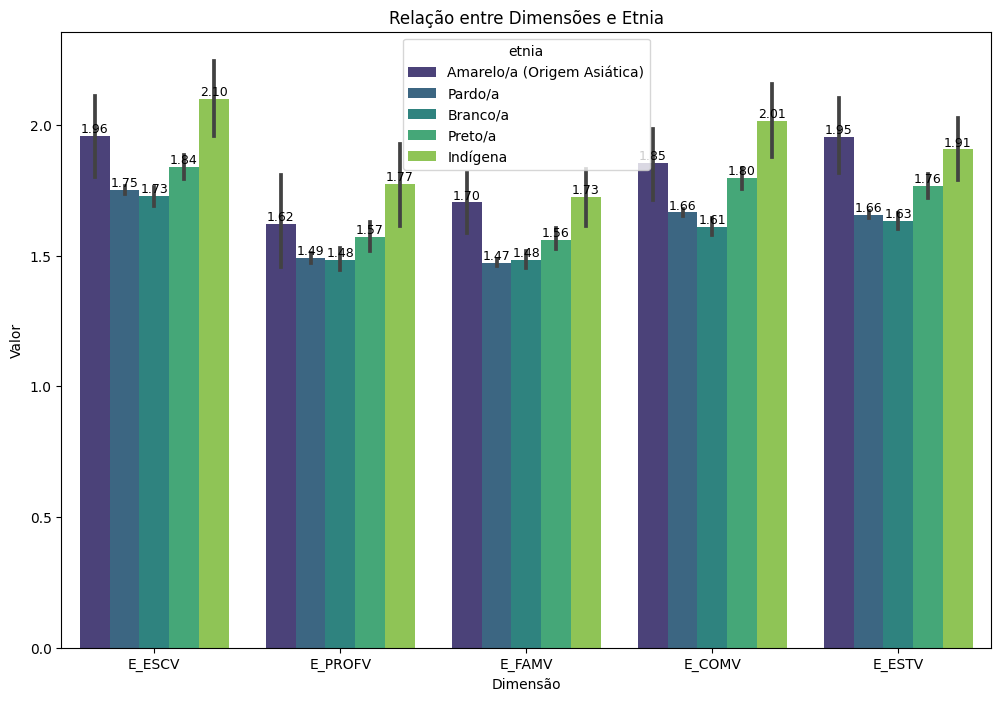
\includegraphics[width=0.8\textwidth]{Textuais/Imagens/Filé/output.png}
%     \caption{Relação entre dimensões e etnia dos estudantes}
%     \label{fig:dimensoes-etnia}
% \end{figure}

% \begin{figure}[ht!]
%     \centering
%     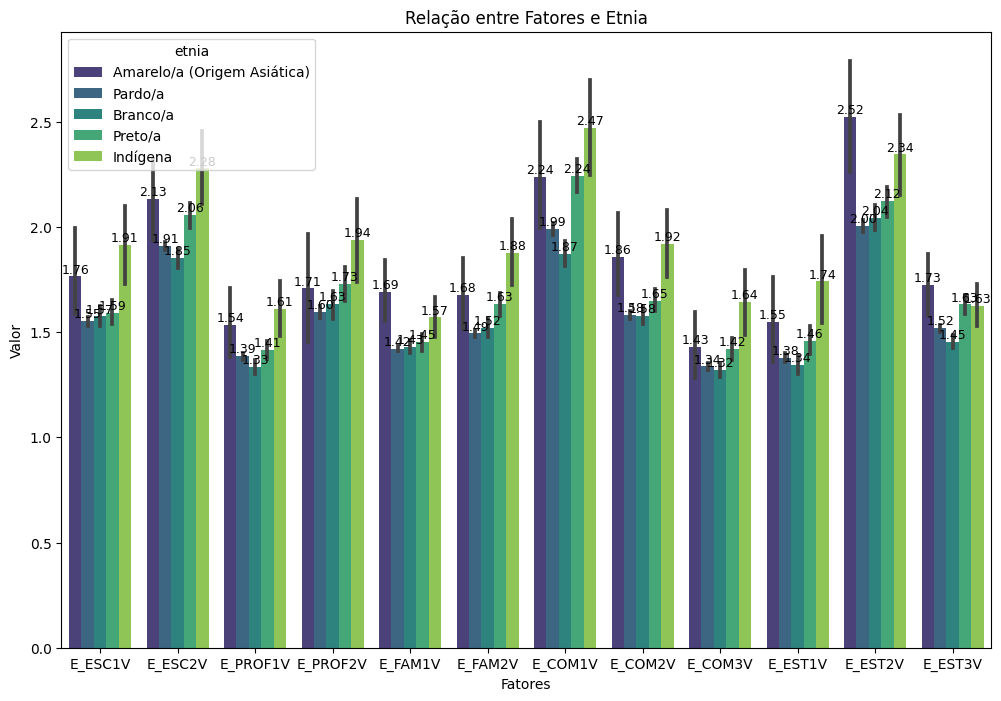
\includegraphics[width=0.8\textwidth]{Textuais/Imagens/Filé/output1.png}
%     \caption{Relação entre fatores e etnia dos estudantes}
%     \label{fig:fatores-etnia}
% \end{figure}

% \begin{figure}[ht!]
%     \centering
%     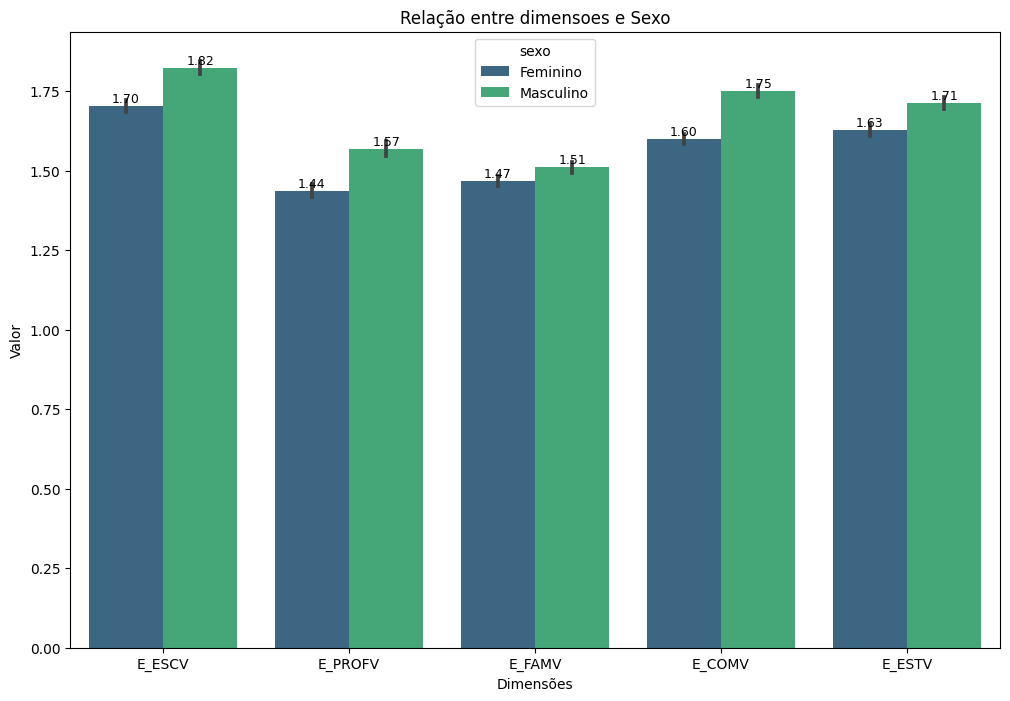
\includegraphics[width=0.8\textwidth]{Textuais/Imagens/Filé/output2.png}
%     \caption{Relação entre dimensões e sexo dos estudantes}
%     \label{fig:dimensoes-sexo}
% \end{figure}

% \begin{figure}[ht!]
%     \centering
%     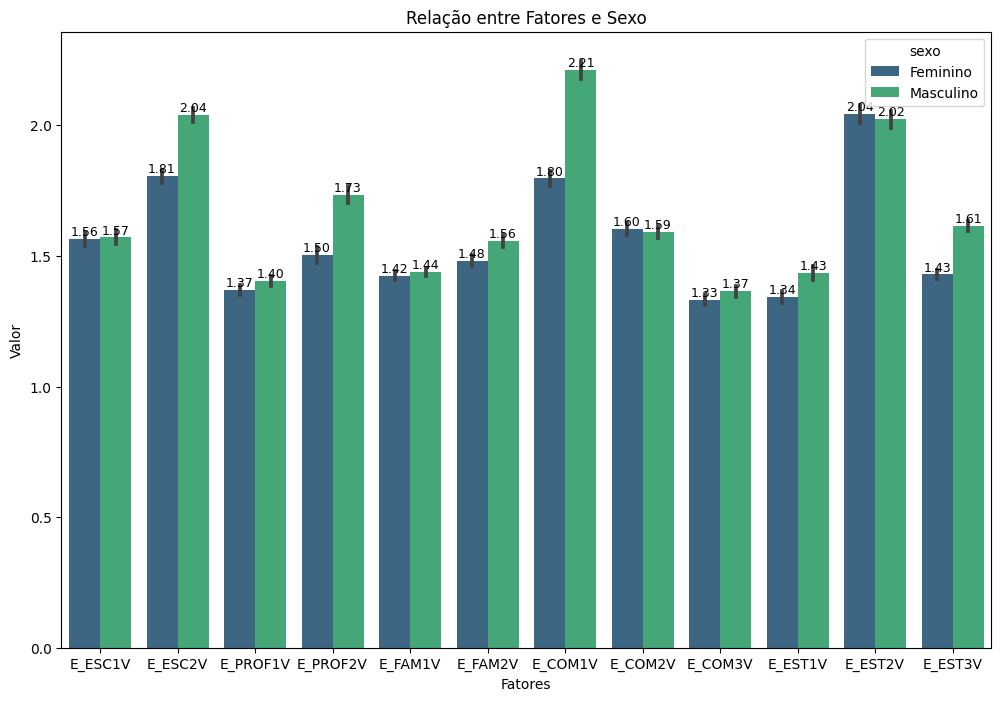
\includegraphics[width=0.8\textwidth]{Textuais/Imagens/Filé/output3.png}
%     \caption{Relação entre fatores e sexo dos estudantes}
%     \label{fig:fatores-sexo}
% \end{figure}

% \begin{figure}[ht!]
%     \centering
%     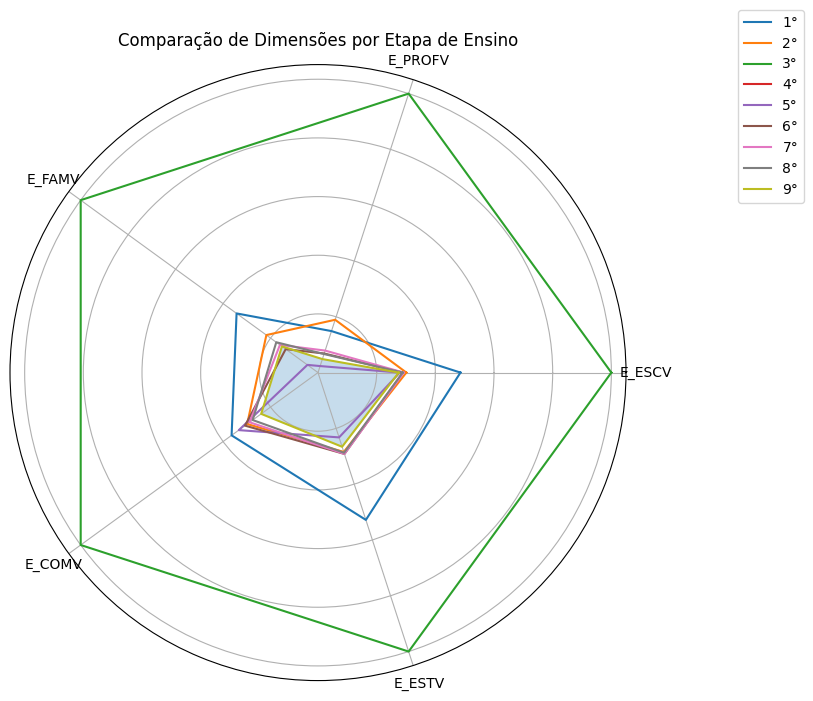
\includegraphics[width=0.8\textwidth]{Textuais/Imagens/Filé/radar_dimensoes.png}
%     \caption{Relação entre dimensões e ano de ensino dos estudantes}
%     \label{fig:dimensoes-anoensino}
% \end{figure}

% \begin{figure}[ht!]
%     \centering
%     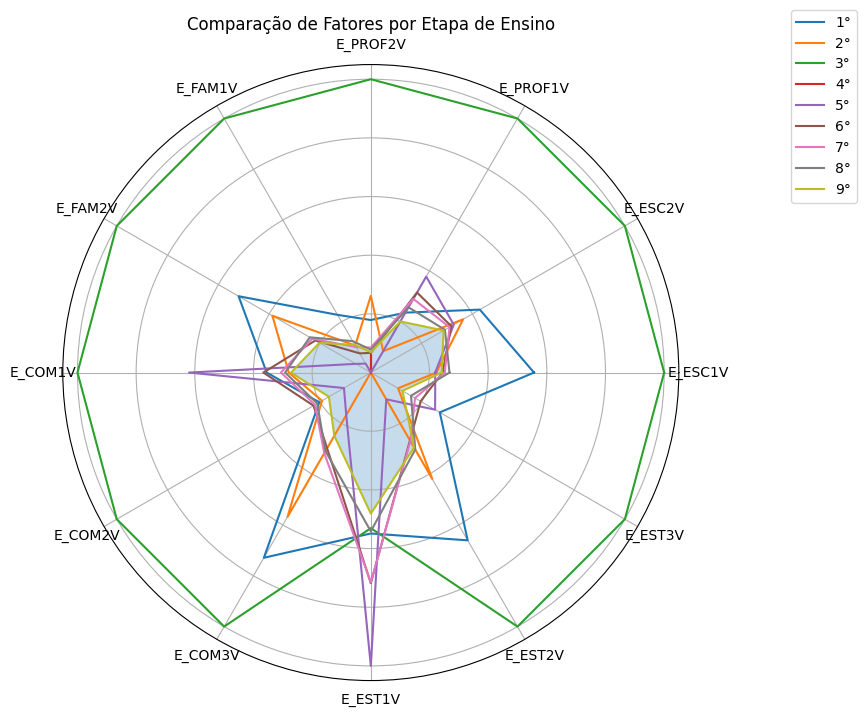
\includegraphics[width=0.8\textwidth]{Textuais/Imagens/Filé/radar_fatores.png}
%     \caption{Relação entre fatores e ano de ensino dos estudantes}
%     \label{fig:fatores-anoensino}
% \end{figure}

% \begin{figure}[ht!]
%     \centering
%     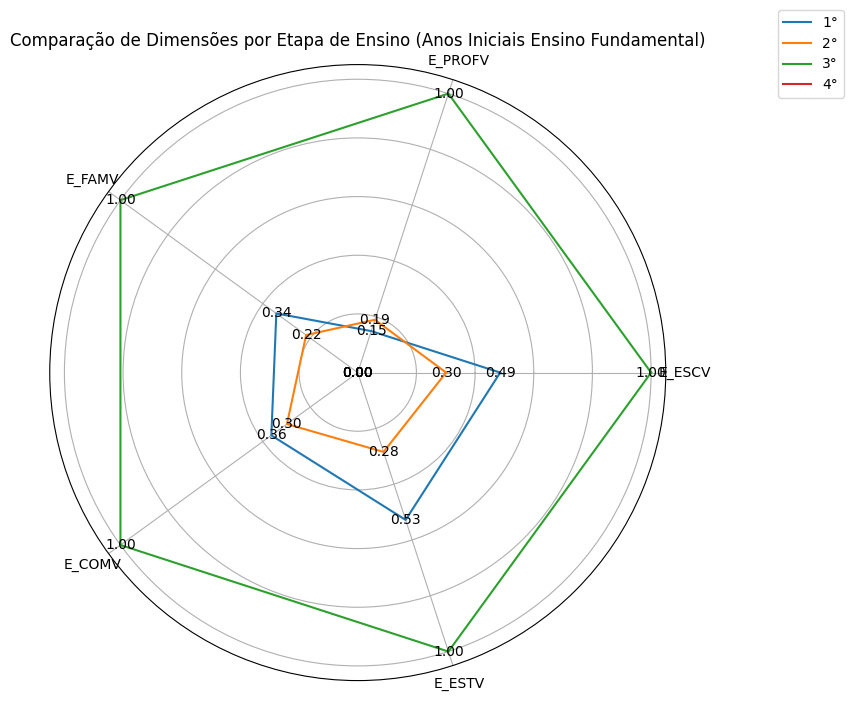
\includegraphics[width=0.4\textwidth]{Textuais/Imagens/Filé/radar_dimensoes_iniciais.png}
%     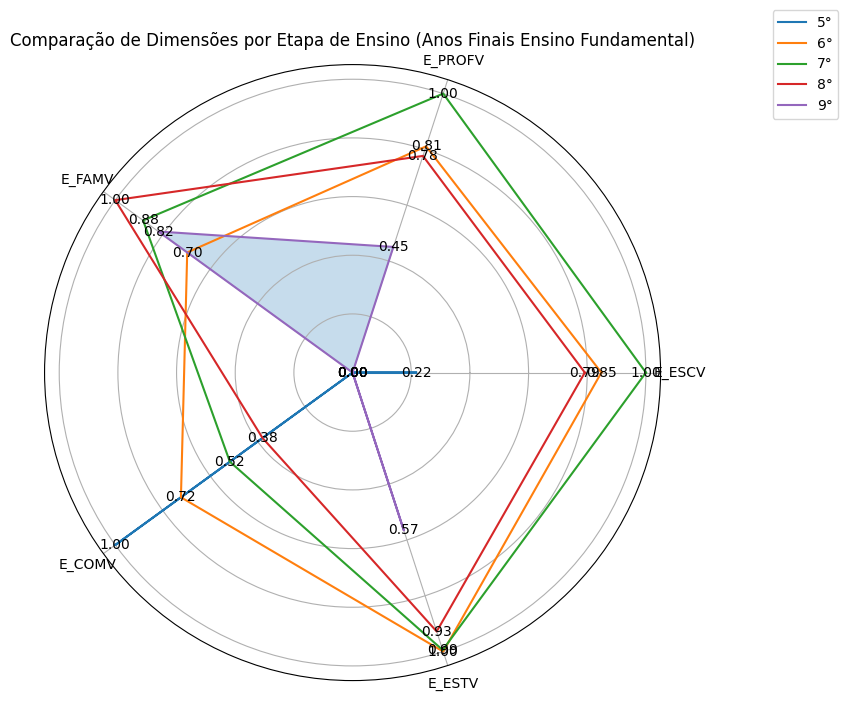
\includegraphics[width=0.4\textwidth]{Textuais/Imagens/Filé/radar_dimensoes_finais.png}
%     \caption{Relação entre dimensões e ano de ensino dos estudantes}
%     \label{fig:dimensoes-anoensino-radar}
% \end{figure}


% \begin{figure}[ht!]
%     \centering
%     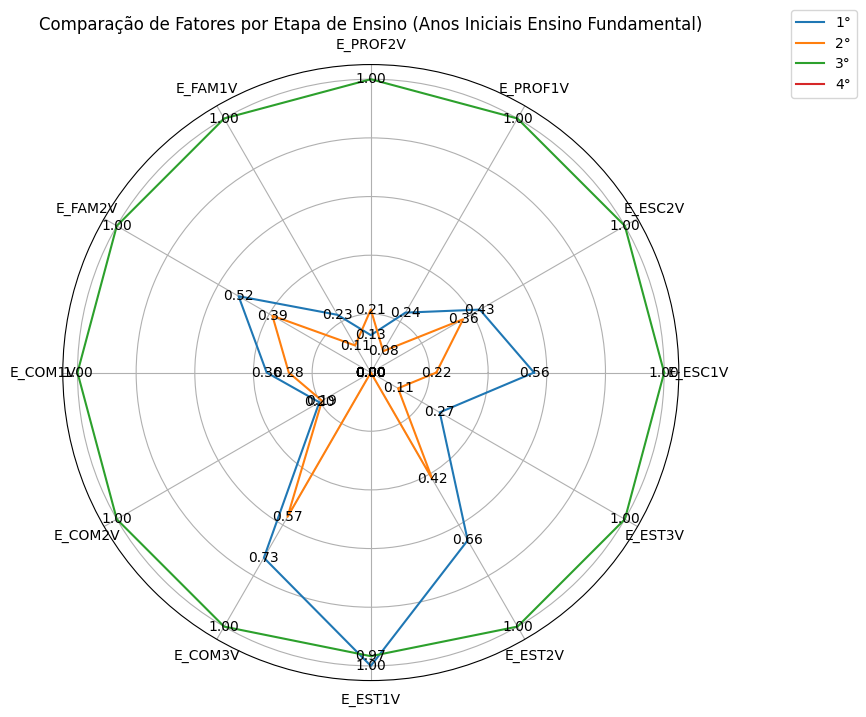
\includegraphics[width=0.4\textwidth]{Textuais/Imagens/Filé/radar_fatores_iniciais.png}
%     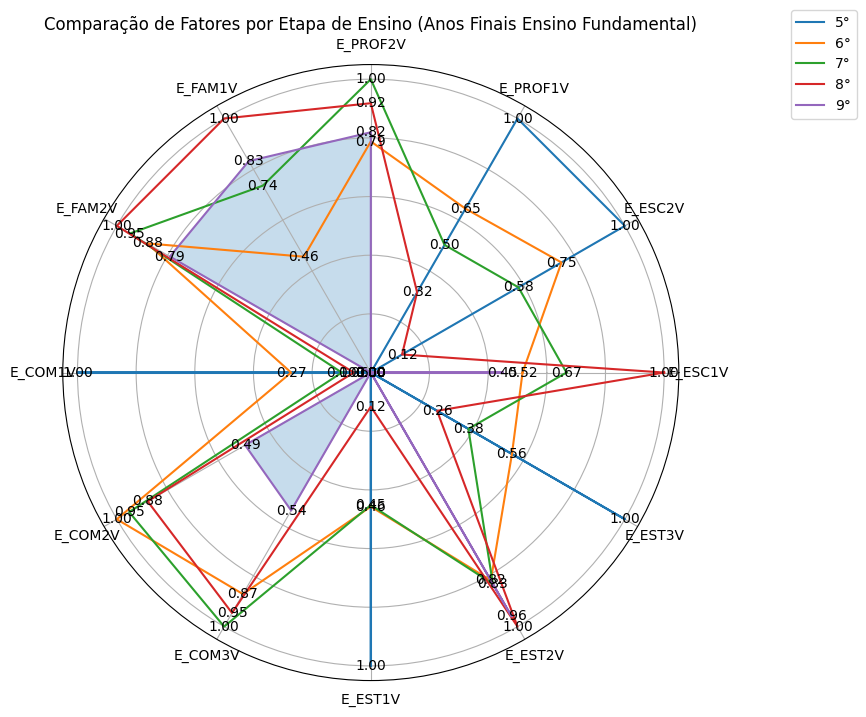
\includegraphics[width=0.4\textwidth]{Textuais/Imagens/Filé/radar_fatores_finais.png}
%     \caption{Relação entre fatores e ano de ensino dos estudantes}
%     \label{fig:fatores-anoensino-radar}
% \end{figure}